\section{Stochastic Integrals}
\label{subsection:stochastic-integrals}
\subsection{Motivation}
Suppose that we want to model the stock price where the time points are in the interval $[0,T]$. We firstly consider a discrete case where $T \in \NN$ and the intermediate time points are $t_n = n, n \in \{0,\ldots, T\}$. Let $p_0$ be the initial stock price at time $t_0$. We wish to establish the formula for the stock price at each time $t_n = n, n \in \{0,\ldots, T\}$ in a nondeterministic way, due to market uncertainty. We can instead formulate the evolution of the price over each time step. Let $\{X_n\}_{n=0}^T$ be a stochastic process where $X_n$ is the price at time $t_n=n$, we have

\begin{equation}
  \begin{cases}
    X_0= p_0 \\
    X_{n+1} - X_n = b(X_n,n) + \sigma(X_n,n)\cdot \texttt{noise}, \,\,\,n\in \{0,\cdots, T-1\},
  \end{cases}
\end{equation}

where $b,\sigma:\RR\times\NN\to\RR$. We select the standard normal random variable for this noise
$$\texttt{noise}:= Z_{n} = W_{n+1}-W_n \sim \N(0,1),$$

by which we hypothesized that if the noise acts more complicatedly, then we can adjust $\sigma(X_n,n)$ to be $\hat{\sigma}(X_n,n)$ such that
$$\sigma(X_n,n)\cdot \texttt{noise} = \hat{\sigma}(X_n,n)(W_{n+1}-W_n) \text{ in } L^2.$$

Our reasonable model is
\begin{equation}
  \label{example:stock-price}
  \begin{cases}
    X_0= p_0 \\
    X_{n+1} - X_n = b(X_n,n) + \sigma(X_n,n)\cdot Z_{n}, \,\,\,n\in \{0,\cdots, T-1\},
  \end{cases}
\end{equation}

\begin{figure}
  \centering
  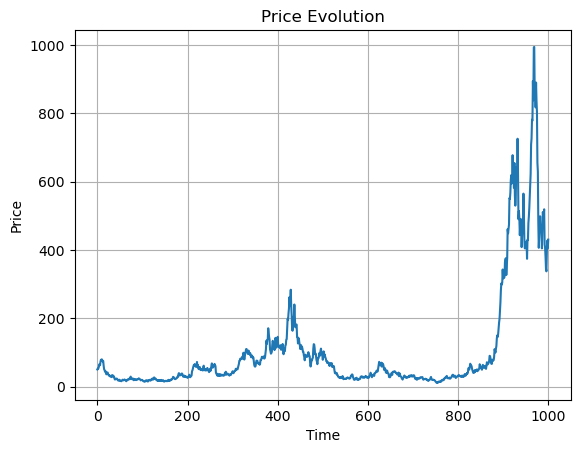
\includegraphics[width=0.7\textwidth]{img/stock-price-sampling.png}
  \vspace{0.25cm}
  \caption[Stock price simulation]{A simulation of stock price evolution by $X_{n+1} - X_n = rX_n + \alpha X_n\cdot Z_{n}$, where $p_0=50, r = 0.005
      \alpha = 0.1$}
\end{figure}

We want to generalize the model in order to predict the price at any time point in $t\in[0,T]$. Let $P^n[0,T]:=\{0=t^n_0<t^n_1<\ldots<t^n_{m_n}=t\}$ be partitions on $[0,T]$ such that $|P^n|\to 0$ as $n\to\infty$ and write
\begin{align*}
  X(t^n_{k+1})- X(t^n_{k})
   & = b(X(t^n_{k}),t^n_{k})(t^n_{k+1} - t^n_{k+1})+ \sigma(X(t^n_{k}),t^n_{k})(W(t^n_{k+1})-W(t^n_{k})) \\
   & = b(X(t^n_{k}),t^n_{k})\Delta t^n_{k} + \sigma(X(t^n_{k}),t^n_{k})\Delta W(t^n_{k}).
\end{align*}

We have
$$X(t)=X(0)+\sum\limits_{k=0}^{m_n-1}  b(X_k^n,t_k^n)\Delta t^n_{k} + \sum\limits_{k=0}^{m_n-1} \sigma(X(t^n_{k}),t^n_{k})\Delta W(t^n_{k}).$$

Let $(\Omega, \F)$ be a measurable space for the stochastic processes $\{X_t\}_{0\le t\le T}$ and $\{W_t\}_{0\le t\le T}$. Set
$$\hat{b}(\omega, t) :=  b(X_t(\omega),t) \text{ and } \hat{\sigma}(\omega, t) := \sigma(X_t(\omega),t), \forall \omega\in\Omega, t\in[0,T].$$

Then
\begin{equation}
  \label{equation:stochastic-limit}
  X(t,\omega)=X(0,\omega)+\sum\limits_{k=0}^{m_n-1}  \hat{b}(\omega, t_k^n)\Delta t^n_{k} + \sum\limits_{k=0}^{m_n-1} \hat{\sigma}(\omega, t_k^n)\Delta W(t^n_{k}), \forall \omega\in\Omega.
\end{equation}

We have
$$\sum\limits_{k=0}^{m_n-1}  \hat{b}(\omega, t_k^n)\Delta t^n_{k}\xrightarrow{n\to\infty} \int\limits_0^t \hat{b}(\omega, t_k^n)\d s$$
as a Riemann sum. When $n\to\infty$, we will prove that the sum $\sum\limits_{k=0}^{m_n-1} \hat{\sigma}(\omega, t_k^n)\Delta W(t^n_{k})$ converges in appropriate sense and adapt the usual integration notation as
\begin{equation}
  \sum\limits_{k=0}^{m_n-1} \hat{\sigma}(\omega, t_k^n)\Delta W(t^n_{k}) \xrightarrow{n\to\infty} \int\limits_0^t \hat{\sigma}(\omega, t_k^n)\d W_s = \int\limits_0^t \sigma(X_s,s)\d W_s.
\end{equation}

\subsection{An Example on the Wiener Process}

In Equation \ref{equation:stochastic-limit}. We have selected in initial points $(t_k^n)_{k=1}^{m_n-1}$ in the partition for the limit of the approximations. Unlike the Riemann integral, each point $\tau_k^n = (1-\lambda) t_k^n + \lambda t_{k+1}^n$, where $\lambda\in[0,1]$, for $k=1,\ldots, m_n-1$ results in different a value of the limit $\sum\limits_{k=0}^{m_n-1} \hat{\sigma}(\tau_k^n, \omega)\Delta W(t^n_{k})$. Let us take a ubiquitous example to emphasize this fact.



\begin{example}
  \label{example:wdw}
  Let $P^n[0,T]:=\{0=t^n_0<t^n_1<\ldots<t^n_{m_n}=T\}$ be partitions on $[0,T]$ such that $|P^n|\to0$ when $n\to\infty$ and $\{W_t\}_{t\in[0,T]}$ be real-valued Wiener process. Calculate the limit
  \begin{equation}
    \lim\limits_{n\to\infty}\sum\limits_{k=0}^{m_n-1} W(\tau_k^n)(W(t^n_{k+1})-W(t^n_{k})),
  \end{equation}
  where
  $\tau_k^n = (1-\lambda) t_k^n + \lambda t_{k+1}^n$ for some $\lambda\in[0,1]$.
\end{example}
% \textcolor{red}{State the result, move the solution to the Appendix}

\begin{solution}
  We have
  \begin{align*}
    R_n
     & = \sum\limits_{k=0}^{m_n-1} W(\tau_k^n)(W(t^n_{k+1})-W({t^n_{k}}))                                                                      \\
     & =
    \sum\limits_{k=0}^{m_n-1}\left[ W(\tau_k^n) - W(t_k^n) + W(t_k^n)\right]\left[W(t^n_{k+1}) - W(\tau_k^n) + W(\tau_k^n) - W(t^n_{k})\right] \\
     & = \underbrace{\sum\limits_{k=0}^{m_n-1}(W(\tau_k^n) - W(t_k^n))(W(t^n_{k+1}) - W(\tau_k^n)) }_{A_n}
    \\
     & \,\,\,\, + \underbrace{\sum\limits_{k=0}^{m_n-1}(W(\tau_k^n) - W(t_k^n))^2  }_{B_n}
    \\
     & \,\,\,\, + \underbrace{ \sum\limits_{k=0}^{m_n-1}(W(t_k^n))(W(t^n_{k+1}) - W(t_k^n))}_{C_n}
  \end{align*}

  Now we study the terms $A_n$, $B_n$ and $C_n$. Let us show that $A_n\to 0$ in $L^2(\Omega)$. Indeed, we have
  \begin{align*}
    \EE[A_n^2]
     & = \EE\left[\left(\sum\limits_{k=0}^{m_n-1}(W(\tau_k^n) - W(t_k^n))(W(t^n_{k+1}) - W(\tau_k^n))\right)^2\right]        \\
     & = \EE\left[\sum\limits_{k=0}^{m_n-1}[(W(\tau_k^n) - W(t_k^n))(W(t^n_{k+1}) - W(\tau_k^n))]^2\right]                   \\
     & \,\,\,\, + \EE\left[\sum\limits_{\substack{k,\ell=0                                                                   \\ k\ne \ell}}^{m_n-1}(W(\tau_k^n) - W(t_k^n))(W(t^n_{k+1}) - W(\tau_k^n))(W(\tau_\ell^n) - W(t_\ell^n))(W(t^n_{\ell+1}) - W(\tau_\ell^n))\right]\\
     & = \sum\limits_{k=0}^{m_n-1}\EE\left[(W(\tau_k^n) - W(t_k^n))^2(W(t^n_{k+1}) - W(\tau_k^n))^2\right]                   \\
     & \,\,\,\, + \sum\limits_{\substack{k,\ell=0                                                                            \\ k\ne \ell}}^{m_n-1}\EE\left[(W(\tau_k^n) - W(t_k^n))(W(t^n_{k+1}) - W(\tau_k^n))(W(\tau_\ell^n) - W(t_\ell^n))(W(t^n_{\ell+1}) - W(\tau_\ell^n))\right]\\
     & = \sum\limits_{k=0}^{m_n-1}\EE\left[(W(\tau_k^n) - W(t_k^n))^2(W(t^n_{k+1}) - W(\tau_k^n))^2\right]                   \\
     & \,\,\,\, + \sum\limits_{\substack{k,\ell=0                                                                            \\ k\ne \ell}}^{m_n-1}\EE\left[(W(\tau_k^n) - W(t_k^n))(W(t^n_{k+1}) - W(\tau_k^n))(W(\tau_\ell^n) - W(t_\ell^n))(W(t^n_{\ell+1}) - W(\tau_\ell^n))\right]\\
     & = \sum\limits_{k=0}^{m_n-1}\EE\left[(W(\tau_k^n) - W(t_k^n))^2\right]  \EE\left[(W(t^n_{k+1}) - W(\tau_k^n))^2\right] \\
     & \,\,\,\, + \sum\limits_{\substack{k,\ell=0                                                                            \\ k\ne \ell}}^{m_n-1}\underbrace{\EE\left[W(\tau_k^n) - W(t_k^n)\right]}_{=0}\EE\left[(W(t^n_{k+1}) - W(\tau_k^n))(W(\tau_\ell^n) - W(t_\ell^n))(W(t^n_{\ell+1}) - W(\tau_\ell^n))\right]\\
     & = \sum\limits_{k=0}^{m_n-1}\EE\left[(W(\tau_k^n) - W(t_k^n))^2\right]  \EE\left[(W(t^n_{k+1}) - W(\tau_k^n))^2\right] \\
     & = \sum\limits_{k=0}^{m_n-1}(1-\lambda)(t_{k+1}^n - t_k)\lambda(t_{k+1}^n - t_k^n)                                     \\
     & \le \lambda(1-\lambda) \sum\limits_{k=0}^{m_n-1}(t_{k+1}^n - t_k)|P^n|                                                \\
     & = \lambda(1-\lambda)T|P^n| \xrightarrow{n\to\infty} 0.
  \end{align*}

  Next, we will show that $B_n\to \lambda T$ in $L^2(\Omega)$.
  \begin{align*}
    \EE[(B_n-\lambda T)^2]
     & = \EE[B_n^2+\lambda^2 T^2 - 2\lambda T B_n]                                                                                                                                            \\
     & = \lambda^2 T^2 - 2\lambda T \EE[ B_n] + \EE[B_n^2]                                                                                                                                    \\
     & = \lambda^2 T^2 - 2\lambda T \sum\limits_{k=0}^{m_n-1} \EE\left[(W(\tau_k^n) - W(t_k^n))^2\right] + \EE\left[\left(\sum\limits_{k=0}^{m_n-1}(W(\tau_k^n) - W(t_k^n))^2\right)^2\right] \\
     & = \lambda^2 T^2 - 2\lambda T \sum\limits_{k=0}^{m_n-1} \lambda (t_{k+1}^n-t_k^n)                                                                                                       \\
     & \,\,\,\, + \sum\limits_{k=0}^{m_n-1}\EE\left[(W(\tau_k^n) - W(t_k^n))^4\right] + \sum\limits_{\substack{k,\ell=0                                                                       \\ k\ne \ell}}^{m_n-1} \EE\left[(W(\tau_k^n) - W(t_k^n))^2(W(\tau_\ell^n) - W(t_\ell^n))^2\right]                                                                                                    \\
     & = -\lambda^2 T^2 + 3\lambda^2\sum\limits_{k=0}^{m_n-1}(t_{k+1}-t_k)^2                                                                                                                  \\
     & \,\,\,\,+ \sum\limits_{\substack{k,\ell=0                                                                                                                                              \\ k\ne \ell}}^{m_n-1} \EE\left[(W(\tau_k^n) - W(t_k^n))^2\right] \EE\left[(W(\tau_\ell^n) - W(t_\ell^n))^2\right] \\
     & = -\lambda^2 T^2 + 3\lambda^2\sum\limits_{k=0}^{m_n-1}(t_{k+1}^n-t_k^n)^2 + \lambda^2\sum\limits_{\substack{k,\ell=0                                                                   \\ k\ne \ell}}^{m_n-1} (t_{k+1}^n-t_k^n)(t_{\ell+1}^n-t_\ell^n) \\
     & = -\lambda^2 T^2 + 2\lambda^2\sum\limits_{k=0}^{m_n-1}(t_{k+1}^n-t_k^n)^2 + \lambda^2\sum\limits_{\substack{k,\ell=0}}^{m_n-1} (t_{k+1}^n-t_k^n)(t_{\ell+1}^n-t_\ell^n)                \\
     & = -\lambda^2 T^2 + 2\lambda^2\sum\limits_{k=0}^{m_n-1}(t_{k+1}^n-t_k^n)^2 + \lambda^2\sum\limits_{\substack{k,\ell=0}}^{m_n-1} (t_{k+1}^n-t_k^n)(t_{\ell+1}^n-t_\ell^n)                \\
     & = 2\lambda^2\sum\limits_{k=0}^{m_n-1}(t_{k+1}^n-t_k^n)^2                                                                                                                               \\
     & \le 2\lambda^2\sum\limits_{k=0}^{m_n-1}|P^n|(t_{k+1}^n-t_k^n)                                                                                                                          \\
     & = 2\lambda^2|P^n|T \xrightarrow{n\to\infty} 0.
  \end{align*}

  The last expression $C_n$ is exactly the case when we choose the initial points.

  Since
  \begin{align*}
    W(t_k^n)(W(t^n_{k+1})-W(t^n_k))
  \end{align*}
  We have
  \begin{align*}
    C_n
     & =\sum\limits_{k=0}^{m_n-1}W(t^n_k)(W(t^n_{k+1})-W(t^n_k))                          \\
     & = \dfrac{1}{2}\left[W^2(t^n_{k+1})-W^2(t^n_k)-(W(t^n_{k+1})-W(^n_k))^2\right]
     & =\dfrac{W^2(T)}{2} -\dfrac{1}{2}\sum\limits_{k=0}^{m_n-1}(W(t^n_{k+1})-W(t^n_k))^2 \\
     & \xrightarrow{n\to\infty} \dfrac{W^2(T)}{2} - \dfrac{T}{2}
  \end{align*}
  Thus,
  $$R_n \xrightarrow{n\to\infty} \dfrac{W^2(T)}{2} + \left(\lambda-\dfrac{1}{2}\right)T.$$
\end{solution}

Two following choices of $\lambda$ are popular in particular
\begin{enumerate}
  \item If $\lambda = 0$, the limit $\lim\limits_{n\to\infty}R_n$ is called an Itô integral, denoted by the conventional integral notation $\int\limits_0^T W\d W$.
  \item If $\lambda = \dfrac{1}{2}$, it is called a Stratonovich integral, denoted by $\int\limits_0^T W\circ\d W$.
\end{enumerate}

In the scope of our project, we concerning about the Itô Integral for later applications on stochastic modeling.

\subsection{Construction of the Itô Integral}

In Equation \ref{equation:stochastic-limit}, we can regard the sum $\sum\limits_{k=0}^{m_n-1} \hat{\sigma}(\omega, t_k^n)\Delta W(t^n_{k})$ as the Itô integral of an elementary function. Similarly to Lebesgue integral construction, we define Itô integral for such class of elementary functions, then generalize the result for a function $\hat{\sigma}(\omega, t)$ satisfying some additional conditions. Now we make consistent definitions for such class of functions.

\begin{definition}[Progressively measurable process]
  Let $\{X_t\}_{t\in[0,T]}$ be a stochastic process adapted to a filtration $\{\F_t\}_{t\in[0,T]}$. Then $\{X_t\}_{t\in[0,T]}$ is said to be progressively measurable if $X_t$ is $\F_t\otimes\B([0,t])$, for any $t\in[0,T]$.
\end{definition}

\begin{definition}[Non-anticipating process]
  Let $W:=\{W_t\}_{t\in[0,T]}$ be a Wiener process, and $\{\W_t\}_{t\in[0,T]}$ be the right-continuous completion of the natural filtration of $W$. Let $\G$ be a $\sigma$-algebra independent of ${\W_t}_{t\in[0,T]}$. Then the non-anticipating filtrations are the ones of the form
  $$\{\sigma(\W_t \cup G)\}_{t\in[0,T]}.$$
  A stochastic process $\{X_t\}_{t\in[0,T]}$ is non-anticipating if it is adapted to some non-anticipating filtration.
\end{definition}

\begin{remark}
  A non-anticipating stochastic process $\{X_t\}_{t\in[0,T]}$ adapted to a sub-$\sigma$-algebra of the natural filtration of a Wiener process. In other words, for any $t\in[0,T]$ we allow $X_t$ to depend on the history of ${\W_t}_{t\in[0,T]}$ up to time $t$, but not the future from time $t$.
\end{remark}

\begin{definition}[Elementary process]
  A progressive, non-anticipating process $\{X_t\}_{t\in[0,T]}$ is elementary if there exists a partition $P[0,T]:=\{0=t_0<t_1<\ldots<t^N=T\}$ such that
  $$X(t) = X(t_n) \text{ if } t \in [t_n, t_{n+1}), \text{ for } j=0,\ldots,N-1.$$
\end{definition}
\begin{remark}
  For an elementary process, the map $t\mapsto X(t,\omega)$ is a step function. We can write an elementary compactly as
  $$X(t) = \sum\limits_{n=0}^{N-1} X(t_n)\mathbf{1}_{[t_n, t_{n+1})}(t),$$
  where $\mathbf{1}$ is the indicator function.
\end{remark}

Denote by $\V := \V[0,T]$ the class of $\L^2$ stochastic processes progressively measurable, non-anticipating. We will prove that any process in $\V$ can be approximated by a sequence of elementary process. Throughout the proofs, we will see reasons why a process must be in class $\V$ so that it is Itô integrable. We follow Equation \ref{equation:stochastic-limit} to define the Itô integral for an elementary process.

\begin{definition}
  Let $\{X_t\}_{t\in[0,T]}$ be an elementary process defined on a partition $P[0,T]:=\{0=t_0<t_1<\ldots<t_N=T\}$. The Itô integral of $\{X_t\}_{t\in[0,T]}$ on $[0,t]$ is
  $$\int\limits_0^t X(t)\d W = \sum\limits_{j=0}^{n-1} X(t_j)(W_{j+1}-W_{j}).$$
  If $\int\limits_0^t X(t)\d W < \infty$, the process $\{X_t\}_{t\in[0,T]}$ is said to be Itô-integrable.
\end{definition}

\begin{lemma}[Approximation of a bounded, continuous process by elementary processes]
  \label{lemma:approximation-1}
  Let $X:=\{X_t\}_{t\in[0,\infty]}$ be a stochastic process that is continuous, progressive, non-anticipating and bounded on $[0, T]$. Then there exists a sequence $(X_n)_{n\in\NN} := (\{X_n(t)\}_{t\in[0,\infty]})_{n\in\NN}$ of bounded, Itô-integrable elementary processes such that
  $$X_n \xrightarrow{n\to\infty} X \text{ in } \L^2.$$
\end{lemma}

\begin{proof}
  Set
  \begin{equation}
    X_n(t) := \sum\limits_{i=1}^\infty X\left(i/2^n\right) \1_{[i/2^n, (i+1)/2^n)}(t).
  \end{equation}
  This is clearly elementary, bounded and square-integrable on $[0, T]$. For any fix $\omega$, we
  $$\int\limits_0^T (X(t,\omega) - X_n(t,\omega))^2 \d t \xrightarrow{n\to\infty} 0,$$
  since $X(t,\omega)$ is continuous. Therefore, the $\L^2$ norm of $X(t) - X_n(t)$, as the expectation of this integral, converges to $0$.
\end{proof}

\begin{lemma}[Approximation of a bounded process by bounded, continuous processes]
  \label{lemma:approximation-2}
  Let $X$ be a stochastic process that is progressive, non-anticipating, bounded on $[0, T]$. Then there exists a sequence $(X_n)_{n\in\NN}$ of continuous, progressive, non-anticipating and bounded on $[0, T]$ processes such that
  $$X_n \xrightarrow{n\to\infty} X \text{ in } \L^2.$$
\end{lemma}
\begin{proof}
  Let $M$ be the bound on the norm of X. For each $n$, pick a probability density $f_n(t):\RR\to\RR$ support is the interval $(-1/n, 0)$. Set
  $$X_n := \int\limits_0^t f_n(s-t) X(s) \d s.$$
  Then $X_n$ is continuous, bounded, progressively measurable, and non-anticipating. Therefore, for any fix $\omega$, we
  $$\int\limits_0^T (X(t,\omega) - X_n(t,\omega))^2 \d t \xrightarrow{n\to\infty} 0,$$
  and so as the $\L^2$ norm of $X(t) - X_n(t)$, as the expectation of this integral.
\end{proof}


\begin{lemma}[Approximation of a $\V$ process by bounded processes]
  \label{lemma:approximation-3}
  Let $X$ be an $\L^2$ stochastic process that is progressive, non-anticipating. Then there exists a sequence $(X_n)_{n\in\NN}$ of progressive, non-anticipating and bounded on $[0, T]$ processes such that
  $$X_n \xrightarrow{n\to\infty} X \text{ in } \L^2.$$
\end{lemma}
\begin{proof}
  Set $X_n(t) = (-n \vee X(t)) \wedge n$. This has the desired properties, and the result follows from dominated convergence.
\end{proof}

\begin{theorem}[Approximation of a $\V$ process by elementary processes]
  Let $X$ be an $\L^2$ stochastic process that is progressive, non-anticipating. Then there exists a sequence $(X_n)_{n\in\NN}$ of bounded, Itô-integrable elementary processes such that
  $$X_n \xrightarrow{n\to\infty} X \text{ in } \L^2.$$
\end{theorem}
\begin{proof}
  The result follows by Lemmas \ref{lemma:approximation-1}, \ref{lemma:approximation-2} and \ref{lemma:approximation-3}.
\end{proof}

\begin{lemma}[Itô isometry for elementary processes]
  Let $\{X_t\}_{t\in[0,T]}$ be a elementary process. Then
  $$\EE\left[\left(\int\limits_0^T X\d W\right)^2\right] = \EE\left[\int\limits_0^T X^2\d W(\omega)\right].$$
\end{lemma}


\begin{proof}
  Let $R_n=\sum\limits_{k=0}^{m_n-1} X(t_k^n)\Delta W(t^n_{k})$. We have
  \begin{align*}
    \EE\left[R_n^2\right]
     & = \EE\left[\sum\limits_{k,\ell = 0}^{m_n-1}X(t_k^n)X(t_\ell^n)\Delta W(t^n_{k}) \Delta W(t^n_{\ell})\right] \\
     & = \sum\limits_{k,\ell = 0}^{m_n-1}\EE\left[X(t_k^n)X(t_\ell^n)\Delta W(t^n_{k}) \Delta W(t^n_{\ell})\right]
  \end{align*}
  If $k \ne \ell$, then $\Delta W(t^n_{k})$ and $\Delta W(t^n_{\ell})$ are independent. Hence,
  \begin{align*}
    \EE\left[X(t_k^n)X(t_\ell^n)\Delta W(t^n_{k}) \Delta W(t^n_{\ell})\right]
     & = \EE\left[X(t_k^n)X(t_\ell^n)\Delta W(t^n_{k})\right]\EE\left[\Delta W(t^n_{\ell})\right] \\
     & =0.
  \end{align*}

  If $k = \ell$, then
  \begin{align*}
    \EE\left[X(t_k^n)X(t_\ell^n)\Delta W(t^n_{k}) \Delta W(t^n_{\ell})\right]
     & =\EE\left[X^2(t_k^n)\right] \EE\left[\Delta W(t^n_{k})^2\right] \\
     & = \EE\left[X^2(t_k^n)\right] (t_{k+1}^n-t_k^n).
  \end{align*}
  Therefore,
  \begin{align*}
    \EE\left[R_n^2\right]
     & =\sum\limits_{k}^{m_n-1} \EE\left[X^2(t_k^n)\right] (t_{k+1}^n-t_k^n)
  \end{align*}
  Taking the limits when $n\to\infty$, we complete the proof.
\end{proof}

\begin{theorem}[Itô integrals of approximating elementary processes converge]
  Let $(X_n)_{n\in\NN}$ be a sequence of $\V$ elementary processes converging to $X$ in $\L^2$. Then the sequence
  $$R_n(X) = \lim\limits_{n\to\infty}\int\limits_0^T X_n\d W$$
  converges in $L^2$. Moreover, this limit is the same for any such approximating sequence $(X_n)$.
\end{theorem}

% \begin{proof}

% \end{proof}

\begin{definition}
  Let $X\in \V$. The Itô integral of $X$ is defined by
  \begin{equation}
    \int\limits_0^T X\d W =  \lim\limits_{n\to\infty}\int\limits_0^T X_n\d W,
  \end{equation}
  where $(\{X_n(t)\}_{t\in[0,T]})_{n\in\NN}$ is a sequence of elementary functions such that
  $$X_n \xrightarrow{n\to\infty} X \text{ in } \L^2.$$
\end{definition}

\begin{theorem}[Properties of Itô integral]
  \label{theorem:prop}
  For all constants $a,b\in\RR$ and $\sigma,H\in\mathcal{V}(S,T)$, we have
  \begin{enumerate}
    \item Linearity: $\int\limits_{S}^T(aG+bH)\d W = a\int\limits_{S}^TG\d W+b\int\limits_{S}^TH\d W$.
    \item $\EE\left[\int\limits_{S}^TG\d W\right]=0$.
    \item Itô isometry: $\EE\left[\left(\int\limits_{S}^TG\d W\right)^2\right]=\EE\left[\int\limits_{S}^TG^2\d t\right]$.
    \item $\EE\left[\int\limits_{S}^TG\d W\int\limits_{S}^TH\d W\right]=\EE\left[\int\limits_{S}^TGH\d W\right]$.
  \end{enumerate}
\end{theorem}

With the linearity property, we are able to define multidimensional Itô integral.

\begin{definition}
  Let $\sigma=(G_{ij})$, where $G_{ij}, 1\le i\le n, 1\le j\le m$ be real-valued stochastic processes. Also, $W=(W_j)$, where $W_j,1\le j\le m$ be real-valued Wiener process. Then for some $T\ge S\ge 0$
  \begin{equation}
    \int\limits_S^T \sigma\d W=\int\limits_S^T\begin{pmatrix}
      G_{11} & \cdots  & G_{1m} \\
      \vdots & \ddots & \vdots \\
      G_{n1} & \cdots  & G_{nm}
    \end{pmatrix}\begin{pmatrix}
      \d W_1 \\\vdots\\\d W_m
    \end{pmatrix}
  \end{equation}
  is an $n$-dimensional vector whose $i$th column is the sum of $m$ one-dimensional integrals
  $$\sum\limits_{j=1}^m \int\limits_S^T G_{ij}\d W_k.$$
\end{definition}

\subsection{Itô's Formulas}
Similarly to ordinary differential equations, there are the chain rule and the product rule in SDE calculus.
\begin{theorem}[One-dimensional Itô's chain rule]
  Suppose that $X_t$ has the stochastic differential
  $$\d X = u\d t + v\d W_t.$$
  Let $g\in C^2(\RR\times[0,\infty))$. Then
  $$Y_t=g(X_t,t)$$
  is given by
  \begin{equation}
    \label{equation:1dchainrule}
    \d Y_t=\dfrac{\partial g}{\partial t}(X_t,t)\d t+\dfrac{\partial g}{\partial x}(X_t,t)\d X_t+\dfrac{1}{2}\dfrac{\partial^2 g}{\partial x^2}(X_t,t)\cdot(\d X_t)^2,
  \end{equation}
  where $(\d X_t)^2=(\d X_t)\cdot(\d X_t)$ is computed according to the rules
  $$\d t\cdot\d t = \d t\cdot\d W_t = \d W_t\cdot\d t = 0, \d W_t\cdot\d W_t=\d t.$$
\end{theorem}

\begin{theorem}[One-dimensional Itô's product rule]
  Suppose $\{X_1(t)\}_{[0,T]}$ and $\{X_2(t)\}_{[0,T]}$ satisfy the following SDEs
  $$\begin{cases}
      \d X_1 = b_1\d t+\sigma_1\d W \\
      \d X_2 = b_2\d t+\sigma_2\d W
    \end{cases}(0\le t\le T).$$
  Then
  \begin{equation}
    \label{theorem:ito-product}
    \d (X_1X_2)=X_2\d X_1+X_1\d X_2+\sigma_1\sigma_2\d t
  \end{equation}
\end{theorem}

% \begin{theorem}[Multidimensional Itô's chain rule]
% \label{equation:mdchainrule}
% \end{theorem}


\subsection{Properties of the Itô Process}

\begin{definition}
  Let $b$ be a non-anticipating measurable process, $\sigma$ be Itô-integrable, and $X_0$ be an $L^2$ random variable independent of $W$. Then the integral
  $$X_t := X_0 + \int_0^t b(s) \d s + \int_0^t \sigma(s) dW$$
  is called an Itô process.
\end{definition}

% \begin{theorem}
%   \label{every-ito-process-is-non-anticipating}
%   Every Itô process is non-anticipating.
% \end{theorem}